%%%%%%%% ICML 2021 EXAMPLE LATEX SUBMISSION FILE %%%%%%%%%%%%%%%%%

\documentclass{article}

% Recommended, but optional, packages for figures and better typesetting:
\usepackage{microtype}
\usepackage{graphicx}
\usepackage{subfigure}
\usepackage{booktabs} % for professional tables

% hyperref makes hyperlinks in the resulting PDF.
% If your build breaks (sometimes temporarily if a hyperlink spans a page)
% please comment out the following usepackage line and replace
% \usepackage{icml2021} with \usepackage[nohyperref]{icml2021} above.
\usepackage{hyperref}

% Attempt to make hyperref and algorithmic work together better:
\newcommand{\theHalgorithm}{\arabic{algorithm}}

\usepackage{amsmath,amssymb,amsthm}
\usepackage{bm,fixmath}




%-------------------- COMMANDS
\DeclareMathOperator*{\argmin}{arg\,min}
\DeclareMathOperator*{\minimize}{minimize}
\DeclareMathOperator{\prox}{prox}
\DeclareMathOperator{\fix}{fix}
\DeclareMathOperator{\proj}{proj}

\newtheorem{theorem}{Theorem}[section]
\newtheorem{remark}[theorem]{Remark}

\newcommand{\norm}[1]{\left\lVert#1\right\rVert}

% new math commands
\newcommand{\N}{\mathbb{N}}
\newcommand{\R}{\mathbb{R}}
\newcommand{\f}{\mathbold{f}}
\newcommand{\bdelta}{\mathbold{\delta}}
\newcommand{\transp}{\top}
\newcommand{\bv}{\mathbold{b}}
\newcommand{\e}{\mathbold{e}}
\newcommand{\p}{\mathbold{p}}
\newcommand{\q}{\mathbold{q}}
\newcommand{\tv}{\mathbold{t}}
\newcommand{\x}{\mathbold{x}}
\newcommand{\y}{\mathbold{y}}
\newcommand{\vv}{\mathbold{v}}
\newcommand{\z}{\mathbold{z}}
\newcommand{\xx}{\pmb{\xi}}
\newcommand{\ball}[2]{\mathbb{B}_{#2}(#1)}
\newcommand{\Am}{\mathbold{A}}
\renewcommand{\Im}{\mathbold{I}}
\newcommand{\Pm}{\mathbold{P}}
\newcommand{\cv}{\mathbold{c}}
\newcommand{\I}{\mathcal{I}}
\newcommand{\T}{\mathcal{T}}

\newcommand{\Ts}{T_\mathrm{s}}

\newcommand{\nicola}[1]{{\color{blue}#1}}
\newcommand{\andrea}[1]{{\color{red}[#1]}}


% Use the following line for the initial blind version submitted for review:
\usepackage{icml2021}

% If accepted, instead use the following line for the camera-ready submission:
%\usepackage[accepted]{icml2021}

% The \icmltitle you define below is probably too long as a header.
% Therefore, a short form for the running title is supplied here:
\icmltitlerunning{OpReg-Boost}

\begin{document}

\twocolumn[
\icmltitle{OpReg-Boost: Learning to Accelerate Online Algorithms \\ with Operator Regression}

% It is OKAY to include author information, even for blind
% submissions: the style file will automatically remove it for you
% unless you've provided the [accepted] option to the icml2021
% package.

% List of affiliations: The first argument should be a (short)
% identifier you will use later to specify author affiliations
% Academic affiliations should list Department, University, City, Region, Country
% Industry affiliations should list Company, City, Region, Country

% You can specify symbols, otherwise they are numbered in order.
% Ideally, you should not use this facility. Affiliations will be numbered
% in order of appearance and this is the preferred way.
\icmlsetsymbol{equal}{*}

\begin{icmlauthorlist}
\icmlauthor{Nicola Bastianello}{unipd}
\icmlauthor{Andrea Simonetto}{ibm}
\icmlauthor{Emiliano Dall'Anese}{cu}
\end{icmlauthorlist}

\icmlaffiliation{unipd}{Department of Information Engineering (DEI), University of Padova, Padova, Italy}
\icmlaffiliation{ibm}{IBM Research Europe, Dublin, Ireland}
\icmlaffiliation{cu}{Department of Electrical, Computer, and Energy Engineering (ECEE), University of Colorado Boulder, Boulder, Colorado, USA}

\icmlcorrespondingauthor{Nicola Bastianello}{nicola.bastianello.3@phd.unipd.it}

% You may provide any keywords that you
% find helpful for describing your paper; these are used to populate
% the "keywords" metadata in the PDF but will not be shown in the document
\icmlkeywords{optimization, online optimization, operator theory, regression, acceleration}

\vskip 0.3in
]

% this must go after the closing bracket ] following \twocolumn[ ...

% This command actually creates the footnote in the first column
% listing the affiliations and the copyright notice.
% The command takes one argument, which is text to display at the start of the footnote.
% The \icmlEqualContribution command is standard text for equal contribution.
% Remove it (just {}) if you do not need this facility.

\printAffiliationsAndNotice{}  % leave blank if no need to mention equal contribution
%\printAffiliationsAndNotice{\icmlEqualContribution} % otherwise use the standard text.

\begin{abstract}
We present OpReg-Boost, a novel acceleration scheme to boost the convergence properties and lessen the asymptotical error of online algorithms for time-varying (weakly) convex optimization problems. OpReg-Boost is built to learn the closest algorithm to a given online algorithm that has all the algorithmic properties one needs for fast convergence, and it is based on the concept of operator regression. We show how to compute OpReg-Boost by using a Peaceman-Rachford solver, and further trade-off computations and accuracy with an interpolation-based technique based on alternating projection. Simulation results showcase the \andrea{better/increase/..} properties of OpReg-Boost w.r.t. the more classical \andrea{...}, and its close relative convex-regression-boost (CvxReg-Boost) which is also novel but significantly less performing.  
\end{abstract}


%------------------------------------------------------------------------------
\section{Introduction}\label{sec:introduction}

\andrea{Add others' papers, esp. ML community}

\andrea{Notation to iron}

In recent years, we have witnessed the growing interest in time-varying optimization problems, where the cost function, constraints, or both are parametrized over data streams, and therefore are changing over time~\cite{Jadbabaie2015, SPM}. Notable applications for the machine learning community are subspace tracking for video streaming and online sparse subspace clustering, see~\cite{Asif2014, Akhriev2020, SPM} and references therein. 

Solving time-varying optimization problems with online algorithms amounts to find and track continuously changing optimizers $\x^*(t)$ and optimal values $F^*(t)$. A significant results for discrete-time online algorithms, that sample and solve sequences of time-varying problems at discrete time-instances $t_k$, $k \in N$, is that if the variations of the problem in time are not vanishing, then online algorithms will have an asymptotical error in terms of optimality, depending on those variations~\cite{Besbes2013, Jadbabaie2015, SPM, NaLi2020}\footnote{
%%% Footnote Jadbabaie:
In~\cite{Jadbabaie2015} and subsequent works, these asymptotical error is formulated in terms of a pertinent notion of regret, and the variations in terms of path-length and functional variability.
%%%
}. While errors can be made small, for instance with the use of prediction-correction algorithms~\cite{Dontchev2013, simonetto_time-varying_2020}, the existence of an asymptotical error remains a distinctive feature of online algorithms for time-varying optimization. 

An eye-opening intuition is then to use the existence of said error to one's advantage, by introducing regularizations in the problem formulation that boost the algorithms convergence. In time-varying scenarios, where convergence rate is crucial, often time then one obtains smaller asymptotical error w.r.t. the original problem if one uses regularizations than if they do not. To reiterate, surprisingly, often when one uses pertinent regularizations, \emph{there is no trade-off between accuracy and speed} and regularized problems offer better speed and asymptotical errors w.r.t. the original problem, even though we are modifying the problem formulation~\cite{Simonetto2014d, Bastianello2020asi}.  

By building on this field-defining fact, once can ask what is the best regularization for a time-varying problem at hand? In this paper, we explore this question in two slightly different angles. First, we ask ourselves: 

{\bf (Q1) } \emph{what is the closest problem to a given time-varying problem that has all the functional properties we need for fast convergence?}

This gives rise to convex-regression-based boosting, or CvxReg-Boost. 
 
To fix the ideas in a static setting, let us consider Figure~\ref{fig.1}, where we have depicted a non-convex function $f$, which we can evaluate at specific points (grey dot). The idea behind Q1 and convex-regression-based boosting is then to interpret the functional evaluation as noisy measurements of an underlying true convex function $\hat{f}$, which we want to learn. As long as $f$ and $\hat{f}$ are not dramatically different, the reasoning is that solving the problem of minimizing $\hat{f}$ instead of $f$ will then give us a boost in term of convergence rate and asymptotical error in online algorithm, despite the fact that $f$ and $\hat{f}$ are different. In addition, and for free, since we have some liberty in designing the functional properties of $\hat{f}$ (e.g., Lipschitz constant, strong convexity constant, etc.), we can thoroughly optimize the parameter of the online algorithm, e.g., its stepsize, further boosting convergence.  

Convex regression is however not the only way to learn good problems, and not the best one (as we are going to explore in the simulation section). A better way is operator regression, which stems from the second question we ask: 

{\bf (Q2) } \emph{what is the closest algorithm to a given online algorithm for solving a time-varying problem that has all the algorithmic properties we need for fast convergence?  
}

In Figure~\ref{fig.1}, we have reported the case of a gradient descent algorithm in terms of a fixed point operator $\mathcal{T} = I - \alpha \nabla_{x}f$, with $\alpha>0$ being the stepsize. The idea here is to use evaluations of $\mathcal{T}$ as noisy measurements of a true underlying operator $\hat{\mathcal{T}}$, with useful properties (e.g., a contractive operator). By using $\hat{\mathcal{T}}$ en lieu of $\mathcal{T}$, then one will be able to boost convergence and reduce the asymptotical error, once again, if $\mathcal{T}$ and $\hat{\mathcal{T}}$ are not dramatically different. 

This latter methodology offers the most promise (as we will showcase in simulation) and it is what we call OpReg-Boost (boosting by operator regression). 


\begin{figure}
\centering
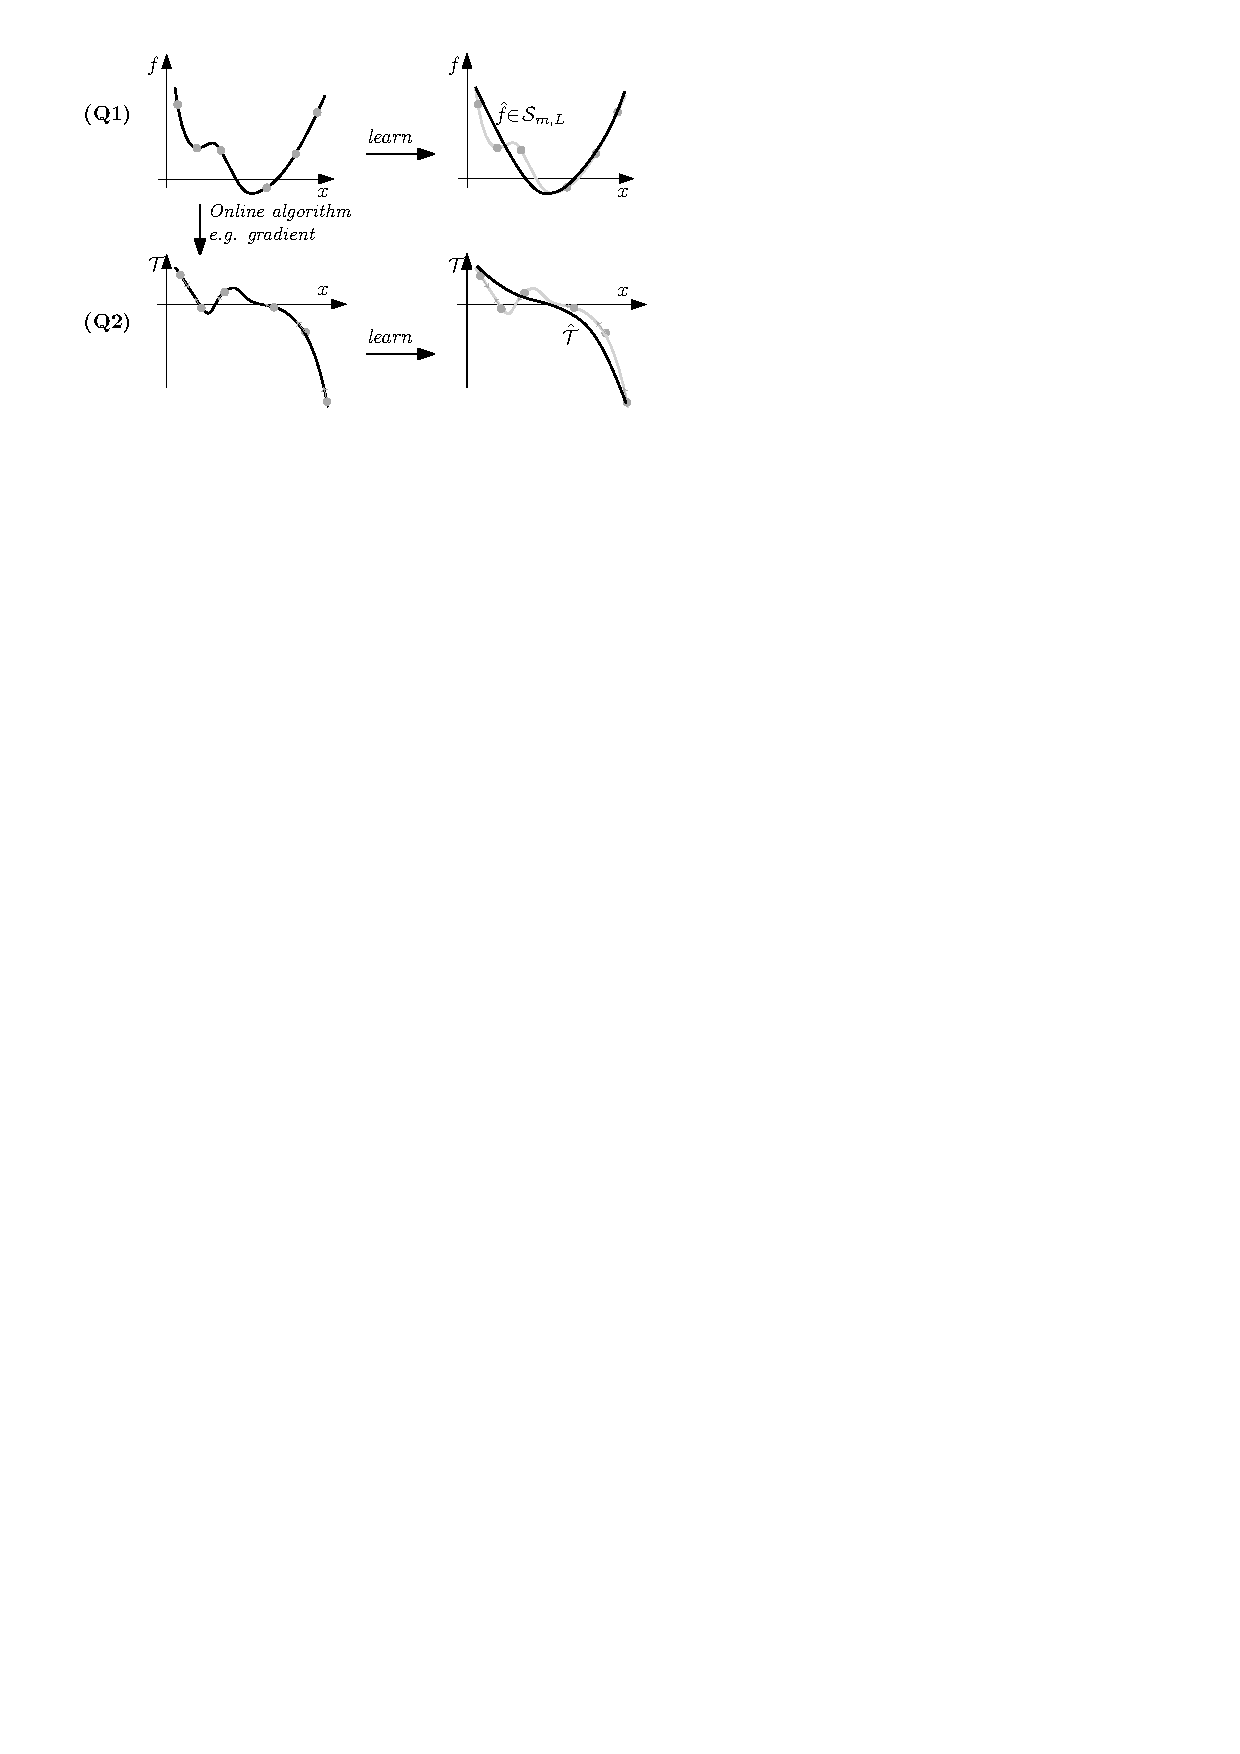
\includegraphics[width=.925\columnwidth]{Figures/explanation}
\caption{The idea of boosting via projection onto the space of ``good'' functions or ``good'' fixed point operators. One can interpret the evaluation of function $f$ or operator $\mathcal{T}$ as noisy evaluations of an underlying ``better'' function or operator, $\hat{f}$ and $\hat{\mathcal{T}}$, respectively, and use the latter to solve the problem instead. This gives rise to convex-regression-based boosting or operation-regression-based boosting (OpReg-Boost).}
\label{fig.1}
\end{figure}

In this paper, we offer the following contributions,
\begin{enumerate}
\item We present two novel regression methods to \emph{learn-project-and-solve} time-varying optimization problems that are not necessarily convex. The methods are based on convex regression and operator regression, and -- especially the latter -- is promising in boosting convergence without introducing a larger asymptotical error. 
%%
\item We present efficient ways to solve the regression problems via a pertinent reformulation of the Peaceman-Rachford splitting (PRS) method. Our PRS method is trivially parallel and allows for a reduction of the per iteration complexity from $O()$ to $O()$, where \andrea{put in the numbers}.  
%%
\item We show how to make use of an 1945 interpolation technique to trade-off accuracy and speed in operation regression, by interpolating the learned operator outside the data points via alternating projections. 
%%
\item We showcase the \andrea{simulation results}
\end{enumerate}

\subsection{Literature review}

\andrea{add ML work}

Time-varying optimization and online algorithms are extensively covered in~\cite{SPM, simonetto_time-varying_2020} and references therein, while a more machine learning approach is offered in~\cite{Jadbabaie2015} and subsequent work. The notion that regularizations help convergence possibly without introducing extra asymptotical error is presented in the papers~\cite{Simonetto2014d, Bastianello2020asi}. While we refer to~\cite{Devolder2011,Nedic2011} for seminal papers close in spirit in the static domain. 

Learning the optimize and regularize is a growing research topic, and we cite~\cite{Nghiem2018,Ongie2020}, as related work, even though not on the problem we are interested in solving here. 

Convex regression is treated extensively in~\cite{Seijo2011,Lim2012,Mazumder2019,Blanchet2019}, while recently being generalized to smooth strongly convex functions~\cite{simonetto_smooth_2021} based on A. Taylor's works~\cite{Taylor2016, Taylor2017}.

Operator regression is a recent and at the same time old topic. We are going to build on the recent work~\cite{ryu_operator_2020} and the F.A. Valentine's 1945 paper~\cite{valentine_lipschitz_1945}.

The acceleration schemes that we compare with are \andrea{Tell and cite, e.g., AA: \cite{pmlr-v119-mai20a}}

\subsection{Notation}

Notation is wherever possible standard. We use the concept of $\mu$-weakly convex function, to indicate a function $f:\R^n \to \R$ that becomes convex by adding the term $\frac{\mu}{2} \|\x-\x_0\|^2_2$, $\mu >0$ (see~\cite{Duchi2018,Davis2019,pmlr-v119-mai20b}). The set of convex functions on $\R^n$ that are $L$-smooth (i.e., have $L$-Lipschitz continuous gradient) and $m$-strongly convex is indicated with $\mathcal{S}_{m,L}(\R^n)$.

An operator $\T: \R^n \to \R^n$ is said to be non-expansive iff $\|T \x - T \y \| \leq \|\x- \y\|$, for all $\x, \y \in \R^n$, whereas it is $\zeta$-contractive, $\zeta\in(0,1)$, iff $\|\T \x - \T \y \| \leq \zeta \|\x- \y\|$, for all $\x, \y \in \R^n$.

We indicate with $\prox_{\alpha g}(\cdot)$ the proximal operator of function $g$ with parameter $\alpha>0$, and with $\proj_{C}(\cdot)$, the projection operator onto the set $C$. 


\section{Problem Formulation}

We are interested in solving the following time-varying optimization problem,
\begin{equation}\label{eq:continuous-time-problem}
	\x^*(t) \in \argmin_{\x \in \R^n} f(\x; t) + g(\x; t) =: F(\x; t)
\end{equation}
where $f : \R^n \times \R_+ \to \R$ is closed, proper, and $\mu$-weakly convex, whereas $g : \R^n \times \R_+ \to \R \cup \{ +\infty \}$ is closed, convex and proper function, optionally with $g \equiv 0$. Upon sampling the problem at discrete time instances $t_k$, we then obtain the sequence of time-invariant problems,
\begin{equation}\label{eq:base-problem}
	\x^*(t_k) \in \argmin_{\x \in \R^n} f(\x; t_k) + g(\x; t_k), \qquad k \in \N. 
\end{equation}
The overarching goal of time-varying optimization is to set up an online algorithm $\mathcal{A}$ that generate a sequence of approximate optimizers $\{\x_k\}_{k\in \N}$, such that the asymptotical tracking error
\begin{equation}
\limsup_{k \to \infty}  \|\x_k - \x^*(t_k)\|,
\end{equation}
is as small as possible. The main blanket assumption is that there exists an optimizer trajectory $\x^*(t)$ such that,
\begin{equation}
\|\x^*(t_{k+1}) - \x^*(t_k)\| \leq \Delta < +\infty, \qquad k \in \N,
\end{equation}
which means that the optimizers can be tracked. 

To fix the ideas, we focus here on online algorithms of the forward-backward type, i.e., for each $t_{k+1}$ we update the sequence $\{\x_k\}_{k \in N}$ as,
\begin{equation}\label{eq:fb}
\x_{k+1} = \prox_{\alpha g(\cdot, t_{k+1})} (\x_{k} - \alpha \nabla_{\x} f(\x_{k}; t_{k+1})), \quad k \in \N.
\end{equation}
Note that the sequence generated by~\eqref{eq:fb} could not converge in general (for a generic non-convex $f$), but it is not important for us, since we are going to regularize either the function $f$ or the algorithm $\mathcal{A}$ so to have converging sequences. 

In particular, we know that for a function $f$ that is in $\mathcal{S}_{m,L}(\R^n)$ uniformly in $k$, then~\eqref{eq:fb} can obtain linear convergence to the asymptotical error bound $\limsup_{k\to\infty} \|\x^*(t_{k+1}) - \x^*(t_k)\| \leq \gamma\Delta/(1-\gamma)$, with optimal $\gamma = \frac{L-m}{L+m}$; much weaker results hold for the general convex case~\cite{Simonetto20XX}. 

Another important result is that even a simple Tikhonov regularization $+ \frac{w}{2} \|x\|^2_2$, transforming the above $f \in \mathcal{S}_{m,L}(\R^n)$ to $f' \in \mathcal{S}_{m',L'}(\R^n)$ with a better $\gamma'<\gamma$, could allow for a boost in convergence and reducing the upper bound on the asymptotical error. In fact, if the optimizers of the true function $F = f+g$ and regularized function $F' = f'+g$ are never farther apart than $e_{\x}$, then the asymptotical error for an algorithm on $F'$ is $\gamma'\Delta'/(1-\gamma') + e_{\x}$, which can be less than the original $\gamma\Delta/(1-\gamma)$.   

\andrea{say something more, change above ..?}

With this in place, our two main research questions are
\begin{itemize}
\item {\bf Q1.} Can we project the weakly convex function $f$ onto $\mathcal{S}_{m,L}(\R^n)$ and learn a better function $\hat{f}$ that has all the functional properties we need (e.g., smooth strong convexity) and use that to solve the problem instead?

\item {\bf Q2.} Can we project the fixed point operator of the algorithm we use $\mathcal{T}$ onto the set of contracting operators, learn a better operator $\hat{\mathcal{T}}$, and use that to solve the problem instead?

\end{itemize}

In the following, we will explore both Q1 and Q2, with a special emphasis on Q2, since it provides better results in simulations. 

\section{Q1. Convex Regression}

We briefly introduce here the concept of convex regression, while we leave the main technical details to~\cite{Mazumder2019,simonetto_smooth_2021}. Suppose one has collected $\ell$ noisy measurements of a convex function $\varphi(\x): \R^n \to \R$ (say $y_i$) at points $\x_i \in \R^n$, $i \in I_{\ell}$, and (optionally) its gradients $\nabla_{\x} \varphi(\x_i)$. Then convex regression is a least-squares approach to estimate the generating function based on the measurements. Formally, letting $\varphi \in \mathcal{S}_{m,L}(\R^n)$, then one would like to solve the infinite-dimensional problem, 
\begin{equation}\label{eq.inf}
\hat{\varphi}_{\ell} \in \argmin_{\psi \in \mathcal{S}_{m, L}(\R^n)}\Big\{ \sum_{i\in I_{\ell}} (y_i - \psi(\x_i))^2 + \|\z_i - \nabla_{\x} \psi(\x_i)\|^2 \Big\} \,,
\end{equation}
where $y_i$ and $\z_i$ are the measurements of the function and the gradients at the data points. 

The problem can be then equivalently decomposed into an estimation on the data points, to find the true function values and gradients at the data point ($\f = [\varphi_i]_{i \in I_{\ell}}$, $\bdelta = [\nabla \varphi_i]_{i \in I_{\ell}}$) which turns out to be a convex quadratically constrained quadratic program, 
\begin{subequations}\label{socp}
\begin{eqnarray}
(\f^*, \bdelta^*) &&\hskip-.5cm= \argmin_{\f\in\R^\ell\!,~ \bdelta \in\R^{n\ell}} \sum_{i\in I_{\ell}} (y_i - \varphi_i)^2 + \|\z_i - \bdelta_i \|^2 \\
\mathrm{s.t.:} &&
\varphi_i - \varphi_j - \bdelta_j^\transp (\x_i - \x_j) \geq \\ && \hskip-5mm \frac{1}{2(1 - m/L)}\left(\frac{1}{L}\|\bdelta_i - \bdelta_j \|^2_2 + m \|\x_i - \x_j\|_2^2 \right. \nonumber \\ && \hskip-5mm \left. - 2 \frac{m}{L} (\bdelta_j-\bdelta_i)^\transp (\x_j - \x_i) \right), \quad \forall i, j \in I_{\ell}. \nonumber
\end{eqnarray} 
\end{subequations}

And an interpolation scheme, that extends the point estimate over the whole space maintaining the functional properties, 
\begin{equation}\label{interp}
\hat{\varphi}_{\ell}(\x) = \mathrm{conv}(p_i(\x)) + \frac{m}{2} \|\x\|^2_2 \in \mathcal{S}_{m,L}(\R^n),
\end{equation}
where
\begin{multline}
p_i(\x) := \frac{L-m}{2} \| {\x} - \x_i\|_2^2 + (\bdelta_i^*-m \x_i)^\transp \x + \\ - \bdelta_i^{*,\transp} \x_i + f_i^* + m/2\|\x_i\|_2^2,
\end{multline}
and where $\mathrm{conv}(\cdot)$ indicates the convex hull.  

Then, to solve Q1, one could consider, for each time $t_k$, a number of evaluations of the function $f(\x; t_k)$ (and optionally its gradients) as noisy measurements of an underlying convex function $\hat{f}_k \in \mathcal{S}_{m,L}(\R^n)$ and using the least-squares approach above to \emph{project} function $f(\cdot; t_k)$ onto the space of ``good'' functions $\mathcal{S}_{m,L}(\R^n)$. Then, one can use the estimated function $\hat{f}_k$ and its estimated gradients to perform a step of the algorithm. 

We include in the appendix all the technical details of such CvxReg-Boost algorithm, while we focus now on solving Q2 via operator regression, which is ultimately better performing. 

\andrea{I think it's not super clear-- Add the algorithm here and the explanation of the compl. complexity and other in the appendix ? }





%------------------------------------------------------------------------------
\section{Q2. Operator Regression}\label{sec:opreg}

\andrea{Decide $k$ or $k+1$}

A slightly different approach to convex regression is to look at the algorithm directly, instead of the function. First of all, we remind the reader that any algorithm can be seen as an operator that maps the current approximate optimizer $\x_k$ into a new approximate optimizer $\x_{k+1}$. For example, a gradient algorithm of the form,
\begin{equation}
\x_{k+1} = \x_k - \alpha \nabla_{\x} f(\x_k; t_k) \equiv \underbrace{(I - \alpha \nabla_{x}f_k)}_{=:\T_k} (\x_k)
\end{equation}
where $\T_k: \R^n \to \R^n$ is the gradient algorithm operator. Interpreting algorithms as operators (possibly averaged, monotone, etc.) has been extremely fruitful for characterizing their convergence properties~\cite{Rockafellar1976, Eckstein1989, bauschke_convex_2017,Ryu2015,Sherson2018}.

The counterpart of a smooth strongly convex function $\varphi_k$ in convex regression, is an operator that is contracting, i.e., $\|\T_k \x - \T_k \y\| \leq \zeta \|\x - \y\|$ for all $\x, \y \in \R^n$ and $\zeta \in (0,1)$. In fact, while $L$-smooth $m$-strongly convex functions give rise to gradient operators that are $..$-contracting, the space of contracting operators is larger (i.e., a function $f$ that is not strongly convex could in principle give rise to a contracting operator~\cite{linear}). 

The key idea now is to interpret evaluations of $\T_k$ as measurements of a true underlying contracting operator that we want to estimate. 
 
% GENERAL PROBLEM.. 
% First, on the data points

First of all, using Fact~2.2 in \cite{ryu_operator_2020}, we know that an operator $\T$ is $\zeta$-contractive interpolable (and therefore extensible to the whole space) if and only if it satisfies
\begin{equation}
	\norm{\T \x_i - \T \x_j}^2 \leq \zeta^2 \norm{\x_i - \x_j}^2, \quad \forall i,j \in I_{\ell}, \ i \neq j.
\end{equation}
Therefore, we can define the following convex quadratically constrained quadratic program as our regression problem:
\begin{equation}\label{eq:operator-regression}
\begin{split}
	\hat{\tv} &= \argmin_{ \R^{n\ell} \ni \tv = [\tv_i]_{i \in I_{\ell}}} \frac{1}{2} \sum_{i \in I_{\ell}} \norm{\tv_i - \T_k \x_i}^2 \\
	&\text{s.t.} \ \norm{\tv_i - \tv_j}^2 \leq \zeta^2 \norm{\x_i - \x_j}^2 \ \forall i,j \in I_{\ell}, i \neq j,
\end{split}
\end{equation}
where again the cost function is a least square terms on the ``observations''' and the constraints enforce contractiveness. In particular, the optimal values $\hat{\tv}$ on the data points represent the evaluations of a $\zeta$-contracting operator when applied to those points, i.e., $\hat{\tv}_i = \hat{\T}_k\x_i$.  

To extend the operator outside the data points in the whole space, we can use a 1945 results, and namely the Corollary to Theorem~5 of \cite{valentine_lipschitz_1945}. In particular, we are interested in interpolating a Lipschitz continuous operator (that is, non-expansive or contractive) from a set of evaluations. The data are the pairs $\{ (\x_i, \hat{\tv}_i) \}_{i \in I_{\ell}}$.

By the Corollary to Theorem~5 of \cite{valentine_lipschitz_1945}, we know that a $\zeta$-Lipschitz continuous map $\hat{\T}_k$ can be extended (that is, interpolated) in a new point $\x$, while preserving Lipschitz continuity $\zeta$, by the construction:
\begin{equation}\label{eq:interpolation}
	\hat{\T}_k \x = \begin{cases}
		\hat{\tv}_i & \text{if} \ \x = \x_i \\
		\hat{\tv} \in \bigcap_{i \in I_{\ell}} \ball{\hat{\tv}_i}{\zeta \norm{\x - \x_i}} & \text{otherwise}
	\end{cases}
\end{equation}
where $\ball{\cv}{r} \subset \R^n$ denotes a ball of center $\cv$ and radius $r$. That is, we can interpolate $\hat{\T}_k$ in a new point $\x$ by finding a point in the intersection of the balls centered in $\hat{\tv}_i$ with radius $\zeta \norm{\x - \x_i}$, $i = 1, \ldots, \ell$. Notice that the intersection $\bigcap_{i \in I_{\ell}} \ball{\hat{\tv}_i}{\zeta \norm{\x - \x_i}}$ is guaranteed to be non-empty by Theorem~1 of \cite{valentine_lipschitz_1945}.

By definition $\hat{\tv}$ satisfies
\begin{equation}
	\norm{\hat{\tv} - \hat{\tv_i}} \leq \zeta \norm{\x - \x_i}, \quad \forall i \in I_{\ell},
\end{equation}
which implies that Lipschitz continuity (and contractivity) is preserved.

\andrea{What happens to $\|\tv' - \tv''\|$ for $\x'$ and $\x''$ both interpolated? Say it has to be sequential! }


Interpolating a Lipschitz continuous operator requires therefore finding a point in the intersection of $\ell$ ball sets. In the Appendix [..], we show how to efficiently compute this intersection with the method of alternating projections~\cite{reich_projection_2015}.

\begin{remark}[Important] We notice here that the convex regression and operator regression methods can be used with any starting function $f$, or operator $\mathcal{T}$. However, functions close to be in $\mathcal{S}_{m,L}(\R^n)$ (e.g., smooth $\mu$-weakly convex functions with small $\mu$) and operators close to be $\zeta$-contractive (e.g., strictly non-expansive operators) would allow for more sensible outcomes. A good point to make here is that the cost function of the regression problems~\eqref{socp} and \eqref{eq:operator-regression} measures the distance between the original function or operator to the class one is projecting them onto, thereby offering a proxy for regularization error. Moreover, one can trade-off regularization accuracy and speed tuning the free parameters $m,L$ or $\zeta$. An option for tuning $\zeta$ automatically is explored in the Appendix.
\end{remark}

\subsection{PRS-based solver}

The solution of the convex problem~\eqref{eq:operator-regression} can be obtained by off-the-shelf solvers, but generally the computational complexity can be a limiting factor, since the problem has a number of constraints that scales quadratically with the number of data points $\ell$. In particular, the computational complexity of interior-point methods would scale as $O()$. This is generally the case in non-parametric regression~\cite{.}. 

Here, we propose a trivially parallel tailored-made algorithm that solves~\eqref{eq:operator-regression} more efficiently (formally .. [..]) based on Peaceman-Rachford splitting (PRS).   

The idea is as follows: each pair of data points $i, j \in I_{\ell}$, $i \neq j$, gives rise to one constraint, for a total of $\ell(\ell-1)/2$ constraints. We define the following set of pairs
\begin{equation}
	\mathcal{V} = \left\{ e = (i,j) \ | \ i, j \in I_{\ell}, \ i < j \right\}
\end{equation}
which are ordered (that is, for example we take $(1,2)$ and not $(2,1)$, to avoid counting constraints twice). To each pair $e = (i,j)$ corresponds the constraint $\norm{\tv_i - \tv_j}^2 \leq \zeta^2 \norm{\x_i - \x_j}^2$.

Let $\tv_{i,e}$ and $\tv_{j,e}$ be copies of $\tv_i$ and $\tv_j$ associated to the $e$-th constraint; then we can equivalently reformulate Problem~\eqref{eq:operator-regression} as
\begin{subequations}\label{eq:equivalent-problem}
\begin{align}
	&\min_{\tv_{i,e}, \tv_{j,e}} \frac{1}{2 (\ell-1)} \sum_{e \in \mathcal{V}} \norm{\begin{bmatrix} \tv_{i,e} \\ \tv_{j,e} \end{bmatrix} - \begin{bmatrix} \y_i \\ \y_j \end{bmatrix}}^2 \\
	&\text{s.t.} \ \norm{\tv_{i,e} - \tv_{j,e}}^2 \leq \zeta^2 \norm{\x_i - \x_j}^2 \label{eq:interpolation-constraints} \\
	&\qquad \tv_{i,e} = \tv_{i,e'} \ \forall e, e' | i \sim e, e'. \label{eq:consensus-constraints}
\end{align}
\end{subequations}
Problem~\eqref{eq:equivalent-problem} is a strongly convex problem with convex constraints defined in the variables $\tv_{i,e}$.

Let $\xx$ be the vector stacking all the $\tv_{i,e}$, then the problem is equivalent to
\begin{align*}
	\min_{\xx} \psi(\xx) + \chi(\xx)
\end{align*}
where
$$
	\psi(\xx) = \frac{1}{2(\ell-1)} \norm{\xx - \y}^2 + \psi_1(\xx)
$$
with $\psi_1$ the indicator function imposing~\eqref{eq:interpolation-constraints} and $\xi$ the indicator function imposing the ``consensus'' constraints~\eqref{eq:consensus-constraints}. The problem can then be solved using the Peaceman-Rachford splitting (PRS) characterized by the following updates $\ell \in \mathbb{N}$:
\begin{subequations}
\begin{align}
	&\xx^j = \prox_{\rho \psi}(\z^j) \label{eq:prs-xi} \\
	&\vv^j = \prox_{\rho \chi}(2 \xx^j - \z^j) \\
	&\z^{j+1} = \z^j + \vv^j - \xx^j.
\end{align}
\end{subequations}
The proximal of $\chi$ corresponds to the projection onto the consensus space, and thus can be characterized simply by
$$
	\vv_{i,e}^j = \frac{1}{\ell-1} \sum_{e' | i \sim e'} \left( 2 \tv_{i,e'}^j - \z_{e'}^j\right).
$$
Regarding the proximal of $\psi$, $\psi$ is separable, in the sense that it can be written as
$$
	\psi(\xx) = \sum_{e \in \mathcal{V}} \left[ \frac{1}{2 (\ell-1)} \norm{\begin{bmatrix} \tv_{i,e} \\ \tv_{j,e} \end{bmatrix} - \begin{bmatrix} \y_i \\ \y_j \end{bmatrix}}^2 + \iota_{e}(\tv_{i,e},\tv_{j,e}) \right]
$$
where $\iota_{e}$ denotes the indicator function of~\eqref{eq:interpolation-constraints} \andrea{is it $\psi_1$?}. Therefore, the update~\eqref{eq:prs-xi} can be solved by solving (possibly in parallel) the problems
\begin{equation}\label{eq:local-updates}
\begin{split}
	(\tv_{i,e},\tv_{j,e}) &= \argmin_{\tv_{i,e},\tv_{j,e}} \left\{ \frac{1}{2 (\ell-1)} \norm{\begin{bmatrix} \tv_{i,e} \\ \tv_{j,e} \end{bmatrix} - \begin{bmatrix} \y_i \\ \y_j \end{bmatrix}}^2 + \right.\\ & \left.\qquad \frac{1}{2\rho} \norm{\begin{bmatrix} \tv_{i,e} \\ \tv_{j,e} \end{bmatrix} - \z_e^j}^2 \right\}\\
	&\text{s.t.} \quad \norm{\tv_{i,e} - \tv_{j,e}}^2 \leq \zeta^2 \norm{\x_i - \x_j}^2.
\end{split}
\end{equation}
Problems~\eqref{eq:local-updates} are convex QCQP with one constraint, and can be solved in the dual domain as scalar problems by using Newton's method~\cite{.}, yielding a total computational complexity of $O(..)$ for the solution of~\eqref{.}.

%------------------------------------------------------------------------------
\section{OpReg-Boost}\label{sec:online-opreg}

We are now ready to present our main algorithm. 

Having to deal with composite problems $f(\cdot; t_k) + g(\cdot; t_k)$, we focus here on online algorithms of the forward-backward type, i.e., 
\begin{equation}
\x_{k+1} = \prox_{g_k} (\x_k - \alpha \nabla_{\x} f_k(\x_k)), \quad k \in \N, \alpha >0.
\end{equation}
We let $\T_k = I - \alpha \nabla_{\x} f_k$ be the operator we want to regularize. Since $f$ is not smooth strongly convex in general, $\T_k$ is not contractive (in general). However, since $g_k$ is convex, the prox operator is non-expansive, so that if $\T_k$ were to be contractive then the forward-backward algorithm would be contracting itself and we could have better convergence guarantees. 

Therefore, we are interested in learning a contracting $\hat{\T}_k$ by evaluations of $\T_k$. The OpReg-Boost algorithm can be described as follows. 

\smallskip
\smallskip
\hrule
{\bf OpReg-Boost algorithm}
\smallskip
\hrule
{\bf Required:} number of points $\ell$, stepsize $\alpha$, contraction factor $\zeta$, initial condition $\x_0$.

At each time $t_k$ do:
\begin{enumerate}
	\item Sample a new problem, that is, observe $f(\x; t_k)$ and $g(\x; t_k)$;
	\item Learn the closest contracting operator to $\T_{k}$, say $\hat{\T}_k$ by:
	%%
	\begin{itemize}
		\item Choose $\ell$ points around $\x_k$ including $\x_k$ itself (e.g., adding a zero-mean Gaussian noise term)
		\item Evaluate the operator on the data points: $\tv_i = \T_{k} \x_i$, $i\in I_{\ell}$, i.e., $\tv_i = \x_i - \alpha \nabla_{\x} f(\x_i; t_k)$;
		\item Solve~\eqref{eq:operator-regression} with the PRS-based solver, and output $\hat{\tv}_k = \hat{\T}_k \x_k$,
\end{itemize}
	%%
	\item Apply $\x_{k+1} = \prox_{g_k} (\hat{\T}_k \x_k) = \prox_{g_k} (\hat{\tv}_k) $.
\end{enumerate}
\smallskip
\hrule

A couple of words are now in order. First, the computational complexity of the algorithm is dominated by the operation regression problem~\eqref{eq:operator-regression}, while its number of gradient calls is $\ell$-times the ones of a standard forward-backward algorithm.  At each time $t_k$, we perform $\ell$ gradient evaluations. We remark that $\ell$ can be as small as $5$ in practice. 

Second, as one can see from step 3., there is no need for solving the interpolation problem~\eqref{eq:interpolation}, since the operation regression problem~\eqref{eq:operator-regression} already provides the evaluation of the regularized operator at the data point $\x_k$. 

In an attempt to reduce gradient calls, we present next an interpolated version of OpReg-Boost. 


%------------------------------------------------
\subsection{Interpolated version}

\andrea{Add intro}


\smallskip
\smallskip
\hrule
{\bf OpReg-Boost with interpolation algorithm}
\smallskip
\hrule
{\bf Required:} number of points $\ell$, stepsize $\alpha$, initial condition $\x_0$, interpolation steps $\tau$.

At each time $t_k$ do:
\begin{enumerate}
	\item Sample a new problem, that is, observe $f(\x; t_k)$ and $g(\x; t_k)$;
	\item {\bf IF} $k \,\textrm{mod}\, \tau = 0$ then, 
	\begin{enumerate}
	\item Learn the closest contracting operator to $\T_{k}$, say $\hat{\T}_k$ by:
	%%
	\begin{itemize}
		\item Choose $\ell$ points around $\x_k$ including $\x_k$ itself (e.g., adding a zero-mean Gaussian noise term)
		\item Evaluate the operator on the data points: $\tv_i = \T_{k} \x_i$, $i\in I_{\ell}$, i.e., $\tv_i = \x_i - \alpha \nabla_{\x} f(\x_i; t_k)$;
		\item Solve~\eqref{eq:operator-regression} with the PRS-based solver, and output $\hat{\tv}_k = \hat{\T}_k \x_k$,
\end{itemize}
\end{enumerate}
	{\bf ELSE},
	\begin{enumerate}
	\item Interpolate last available $\hat{\T}_t$ for $\tv_k = \x_k - \alpha \nabla_{\x} f(\x_k; t_k)$ by using~\eqref{eq:interpolation} with the method of alternating projections and output $\hat{\tv}_k$ 
\end{enumerate}
	%%
	\item Apply $\x_{k+1} = \prox_{g_k} (\hat{\tv}_k) $.
\end{enumerate}
\smallskip
\hrule

\andrea{add explanation and closure.}



%------------------------------------------------------------------------------
\section{Numerical Results}\label{sec:numerical}

Wish-list

\begin{itemize}
\item non-negative Least-squares

\item L1 ? 

\item Relative-entropy non-negative regression

\item weakly convex: time-varying phase retrival? (see Convergence of a Stochastic Gradient Method with Momentum for Nonsmooth Nonconvex Optimization)

\end{itemize}

Compare (real-time, gradient/functional calls) with Nesterov, AA, CvxReg-Boost, OpReg-Boost, Gradient descent. Other? (Forward-backward envelope, superMann?)

For the weakly convex one: See Convergence of a Stochastic Gradient Method with Momentum for Nonsmooth Nonconvex Optimization (momentum as described there?)



%------------------------------------------------
\subsection{Simulations set-up}
We consider the following time-varying problem:
\begin{equation}\label{eq:tv-problem}
	\x^*(t_k) = \argmin_{\x \in \R^n} \frac{1}{2} \norm{\Am \x - \bv(t_k)}^2 + w \norm{\x}_1
\end{equation}
with $n = 10$, $\Am$ matrix with maximum and minimum (non-zero) eigenvalues $\sqrt{L} = 10^8$, $\sqrt{\mu} = 1$, and with rank $5$; $\y(t_k)$ has sinusoidal components with $3$ zero components. Due to $\Am$ being rank deficient, the cost $f$ is convex but not strongly so.


%------------------------------------------------
\subsection{Results}




%% FIGURE
%\begin{figure}[ht]
%\vskip 0.2in
%\begin{center}
%\centerline{\includegraphics[width=\columnwidth]{icml_numpapers}}
%\caption{Historical locations and number of accepted papers for International
%Machine Learning Conferences (ICML 1993 -- ICML 2008) and International
%Workshops on Machine Learning (ML 1988 -- ML 1992). At the time this figure was
%produced, the number of accepted papers for ICML 2008 was unknown and instead
%estimated.}
%\label{icml-historical}
%\end{center}
%\vskip -0.2in
%\end{figure}


%% ALGORITHM
%\begin{algorithm}[tb]
%   \caption{Bubble Sort}
%   \label{alg:example}
%\begin{algorithmic}
%   \STATE {\bfseries Input:} data $x_i$, size $m$
%   \REPEAT
%   \STATE Initialize $noChange = true$.
%   \FOR{$i=1$ {\bfseries to} $m-1$}
%   \IF{$x_i > x_{i+1}$}
%   \STATE Swap $x_i$ and $x_{i+1}$
%   \STATE $noChange = false$
%   \ENDIF
%   \ENDFOR
%   \UNTIL{$noChange$ is $true$}
%\end{algorithmic}
%\end{algorithm}

%% TABLE
%\begin{table}[t]
%\caption{Classification accuracies for naive Bayes and flexible
%Bayes on various data sets.}
%\label{sample-table}
%\vskip 0.15in
%\begin{center}
%\begin{small}
%\begin{sc}
%\begin{tabular}{lcccr}
%\toprule
%Data set & Naive & Flexible & Better? \\
%\midrule
%Breast    & 95.9$\pm$ 0.2& 96.7$\pm$ 0.2& $\surd$ \\
%Cleveland & 83.3$\pm$ 0.6& 80.0$\pm$ 0.6& $\times$\\
%Glass2    & 61.9$\pm$ 1.4& 83.8$\pm$ 0.7& $\surd$ \\
%Credit    & 74.8$\pm$ 0.5& 78.3$\pm$ 0.6&         \\
%Horse     & 73.3$\pm$ 0.9& 69.7$\pm$ 1.0& $\times$\\
%Meta      & 67.1$\pm$ 0.6& 76.5$\pm$ 0.5& $\surd$ \\
%Pima      & 75.1$\pm$ 0.6& 73.9$\pm$ 0.5&         \\
%Vehicle   & 44.9$\pm$ 0.6& 61.5$\pm$ 0.4& $\surd$ \\
%\bottomrule
%\end{tabular}
%\end{sc}
%\end{small}
%\end{center}
%\vskip -0.1in
%\end{table}



\newpage 

\bibliography{PaperCollection00,references}
\bibliographystyle{icml2021}


%%%%%%%%%%%%%%%%%%%%%%%%%%%%%%%%%%%%%%%%%%%%%%%%%%%%%%%%%%%%%%%%%%%%%%%%%%%%%%%
\newpage
\appendix

%------------------------------------------------------------------------------
\section{CvxReg-Boost}

\andrea{[Write here cvx reg boost.. and algorithm.]}


\subsection{Optional auto-tuning for $\zeta$ in~\eqref{eq:operator-regression}}

Discretionarily, we can also modify~\eqref{eq:operator-regression} by including $w = \zeta^2$ as an unknown of the regression problem with a penalty $c>0$, which then becomes
\begin{equation}
\begin{split}
	(\hat{\tv}, \hat{w}) &= \argmin_{ \R^{n\ell} \ni \tv = [\tv_i]_{i \in I_{\ell}}, w \in (0,1)} \frac{1}{2} \sum_{i \in I_{\ell}} \norm{\tv_i - \y_i}^2 + \frac{c}{2} w^2 \\
	&\text{s.t.} \ \norm{\tv_i - \tv_j}^2 - w \norm{\x_i - \x_j}^2 \leq 0 \ \forall i,j \in I_{\ell}, i \neq j,
\end{split}
\end{equation}
this way the contraction constant does not need to be specified, and it is \emph{auto-tuned} by the regression.

%------------------------------------------------------------------------------
\section{PRS-Based QCQP solver}
In this section we present a solver for OpReg which can be efficiently parallelized, inspired by the approach in \cite{simonetto_smooth_2021}.

[Maybe here specify the Newton's step?]

%------------------------------------------------------------
\subsection{Local updates}
The problems~\eqref{eq:local-updates} are quadratic programs with quadratic constraints, that is, they can be written in the form
\begin{subequations}
\begin{align}
	&\min_{\xx} \frac{1}{2} \xx^\top \Pm_0 \xx + \langle \q_0, \xx \rangle \\
	&\text{s.t.} \ \frac{1}{2} \xx^\top \Pm_1 \xx + \langle \q_1, \xx \rangle + r_1 \leq 0.
\end{align}
\end{subequations}
In particular, for the cost function we have
$$
	\Pm_0 = \left( \frac{1}{D-1} + \frac{1}{\rho} \right) \Im_{2n}, \quad \q_0 = - \left( \frac{1}{D-1} \begin{bmatrix} \y_i \\ \y_j \end{bmatrix} + \frac{1}{\rho} \z_e^\ell \right)
$$
and for the constraint
$$
	\Pm_1 = 2 \begin{bmatrix} \Im_n & - \Im_n \\ - \Im_n & \Im_n \end{bmatrix}, \quad \q_1 = 0{2n}, \quad r_1 = - \zeta^2 \norm{\x_i - \x_j}^2.
$$


%------------------------------------------------------------------------------
\section{Interpolating a Lipschitz continuous operator}
%%%%%%%%%%%%%%%%%%%%%%%%%%%%%%%%%%%%%%%%%%%%%%%%%%%%%%%%%%%%%%%%%%%%%%%%%%%%%%%
%%% INTERPOLATION
%%%%%%%%%%%%%%%%%%%%%%%%%%%%%%%%%%%%%%%%%%%%%%%%%%%%%%%%%%%%%%%%%%%%%%%%%%%%%%%

We will be discussing possible methods to solve the interpolation problem~\eqref{eq:interpolation} to select the most efficient strategy. Problem~\eqref{eq:interpolation} is a \emph{feasibility problem}, that is, it requires that we find a point in the intersection of closed, convex sets. There are several algorithms for solving this class of problems, \emph{e.g.} the method of alternating projections (MAP) and Peaceman-Rachford splitting, see \cite{reich_projection_2015} for a review.

Moreover, the feasibility problem~\eqref{eq:interpolation} can also be solved using \emph{best approximation methods}, which find the point in the intersection that is closest to a given vector. Of course best approximation problems are more difficult than feasibility ones. The literature on best approximation is very vast, see \emph{e.g.} \cite{reich_projection_2015}, Chapter~30 of \cite{bauschke_convex_2017}, \cite{artacho_new_2018} and references therein.

Finally, given the fact that~\eqref{eq:interpolation} requires a point in the intersection of balls, we may use methods that are tailored to the particular structure of ball sets, \emph{e.g.} \cite{lushchakova_geometric_2020}.

\subsection{Comparison}
The numerical results reported in the here are derived in the following set-up. We generate $\ell$ intersecting ball sets in $\R^n$, with radii randomly picked in $(0, 100)$. The centers of the balls are randomly chosen so that the sets include the origin, and are thus guaranteed to intersect at least in that point.

In Figure~\ref{fig:projection_methods} we report a comparison of three feasibility methods -- alternating projections (MAP), parallel projections (PP), Peaceman-Rachford splitting(PRS) \cite{reich_projection_2015,bauschke_convex_2017} -- and two best approximation methods -- Halpern and Haugazeau methods \cite{bauschke_convex_2017}. The simulations are performed choosing a number of points $\ell = 50$ in dimension $n = 5$.

\begin{figure}[!ht]
\centering
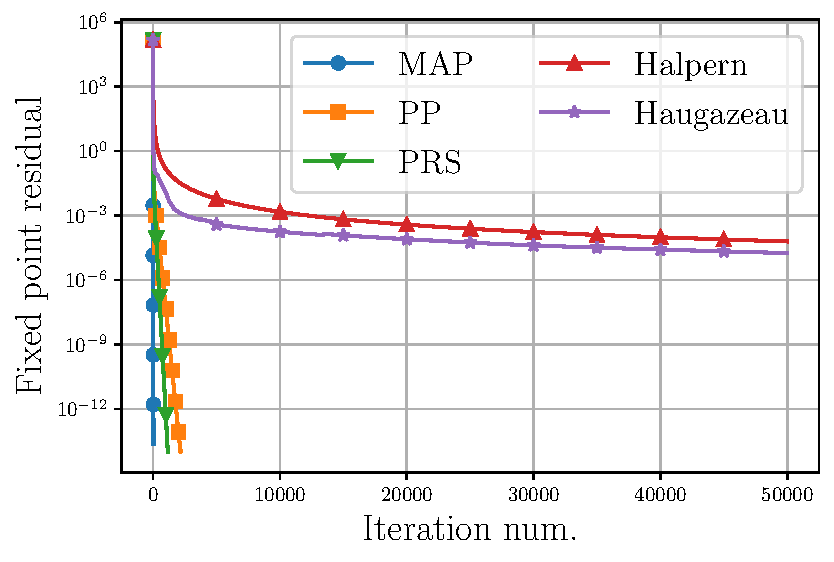
\includegraphics[width = 0.9\columnwidth]{Figures/comparison_projection_methods}
\caption{Comparison of feasibility and best approximation methods.}
\label{fig:projection_methods}
\end{figure}

As we can see, MAP is by far the fastest of the methods, reaching convergence (with tolerance $10^{-14}$) in just $33$ iterations. Parallel projections and Peaceman-Rachford splitting reach convergence in $1930$ and $1036$ iterations, respectively, while the best approximation methods are still far from converging after $50000$ iterations.

MAP not only achieves superior convergence speed, but it is also the simplest of the methods in terms of computational complexity, see \emph{e.g.} \cite{reich_projection_2015}. Therefore we select MAP for our interpolation problem. 

\begin{remark}
Although MAP achieves extremely fast convergence when applied to~\eqref{eq:interpolation}, this is by no means true in general; indeed, it is possible to show that MAP has \emph{arbitrarily slow} convergence in some scenarios, see for example \cite{hundal_alternating_2004,bauschke_characterizing_2009}.
\end{remark}

%------------------------------------------
\subsection{How fast is MAP?}
As shown in the previous section, solving~\eqref{eq:interpolation} using the method of alternating projections is very effective. Recall that the MAP is characterized by the following update
\begin{equation}\label{eq:alternating_projections}
	\x^{j+1} = (\proj_{\ball{\cv_{\ell}}{r_{\ell}}} \circ \cdots \proj_{\ball{\cv_1}{r_1}}) \x^j, \quad j \in \N
\end{equation}
for any initial condition $\x^0 \in \R^n$.

In Figure~\ref{fig:map-histogram} we report an histogram of the number of iterations that MAP required to converge, with $\ell = 100$ and $n = 25$. The histogram is computed using data from $10000$ repetitions, each repetition being characterized by a different set of randomly generated balls.

\begin{figure}[!ht]
\centering
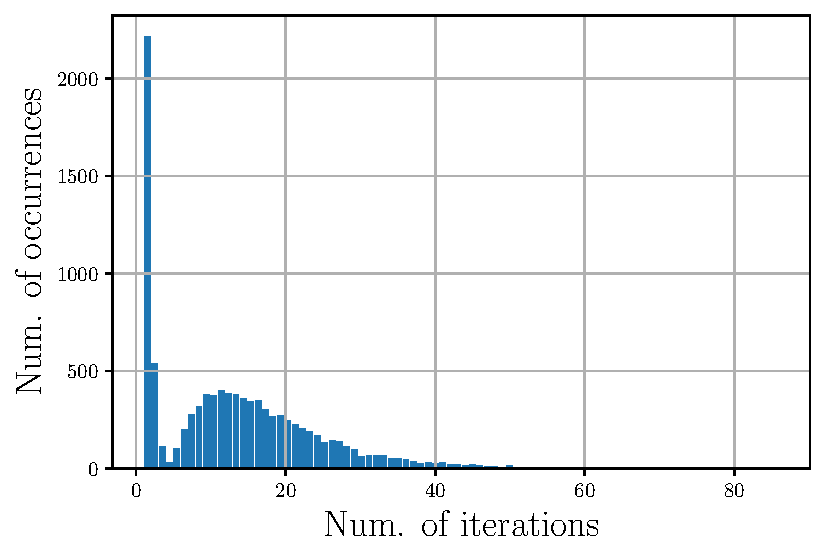
\includegraphics[width = 0.9\columnwidth]{Figures/MAP_histogram}
\caption{Histogram of iterations required by MAP over $10000$ repetitions.}
\label{fig:map-histogram}
\end{figure}

As we can see, in almost one quarter of the repetitions MAP required a single iteration to converge, while the remaining number of iterations occur $\sim 500$ or less. In particular, the maximum number of iterations is $86$, and the mean is approximately $13 \pm 11$.

In Figure~\ref{fig:map-changing-d} instead we evaluate the effect of the number of balls on the speed of MAP. For each value of $\ell$ between $2$ and $100$ we perform $10000$ repetitions of MAP, each repetition being characterized by a different random set of balls.

\begin{figure}[!ht]
\centering
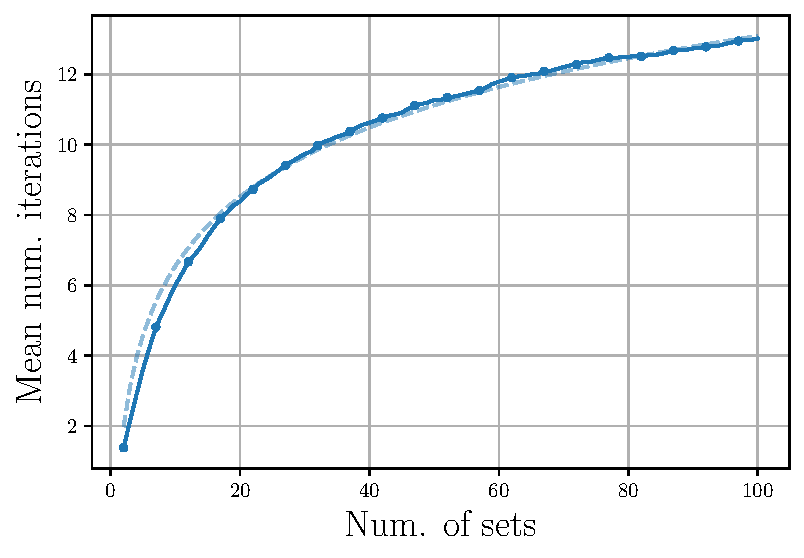
\includegraphics[width = 0.9\columnwidth]{Figures/MAP_changing_d}
\caption{Histogram of iterations required by MAP over $10000$ repetitions.}
\label{fig:map-changing-d}
\end{figure}

As we can see, the mean number of iterations required by MAP grows as the $\log(\ell)$, in particular as $2.84 \log(\ell)$ (dashed curve). Even though a larger number of sets increases the number of iterations, this number is still very small (in mean) even for $\ell = 100$.





%%%%%%%%%%%%%%%%%%%%%%%%%%%%%%%%%%%%%%%%%%%%%%%%%%%%%%%%%%%%%%%%%%%%%%%%%%%%%%%


\end{document}


% This document was modified from the file originally made available by
% Pat Langley and Andrea Danyluk for ICML-2K. This version was created
% by Iain Murray in 2018, and modified by Alexandre Bouchard in
% 2019 and 2021. Previous contributors include Dan Roy, Lise Getoor and Tobias
% Scheffer, which was slightly modified from the 2010 version by
% Thorsten Joachims & Johannes Fuernkranz, slightly modified from the
% 2009 version by Kiri Wagstaff and Sam Roweis's 2008 version, which is
% slightly modified from Prasad Tadepalli's 2007 version which is a
% lightly changed version of the previous year's version by Andrew
% Moore, which was in turn edited from those of Kristian Kersting and
% Codrina Lauth. Alex Smola contributed to the algorithmic style files.